\subsection{Principle Component Analysis}
The Principle Components Analysis (PCA) is an tool that can be used to describe the variance in a data set.

PCA aims to reduce the number of dimension used to represent the features of the data.
This is done by finding the eigenvectors and eigenvalues to the training set and removing some of the components representing the least variance in the data set.
Thus efficiently reducing the dimensions, but still keeping the most significant knowledge about the features.

By selecting the most significant principle components (PC) the data set can be systematically reduced with minimal changes to performance.
In figure \ref{fig:variance} is the variance and accumulated variance shown for the first 20 PC. 
It is seen that the first PC is the most significant and the variance converges towards zero with more PC.

\begin{figure}[H]
\centering
\begin{subfigure}{0.70\textwidth}
\centering
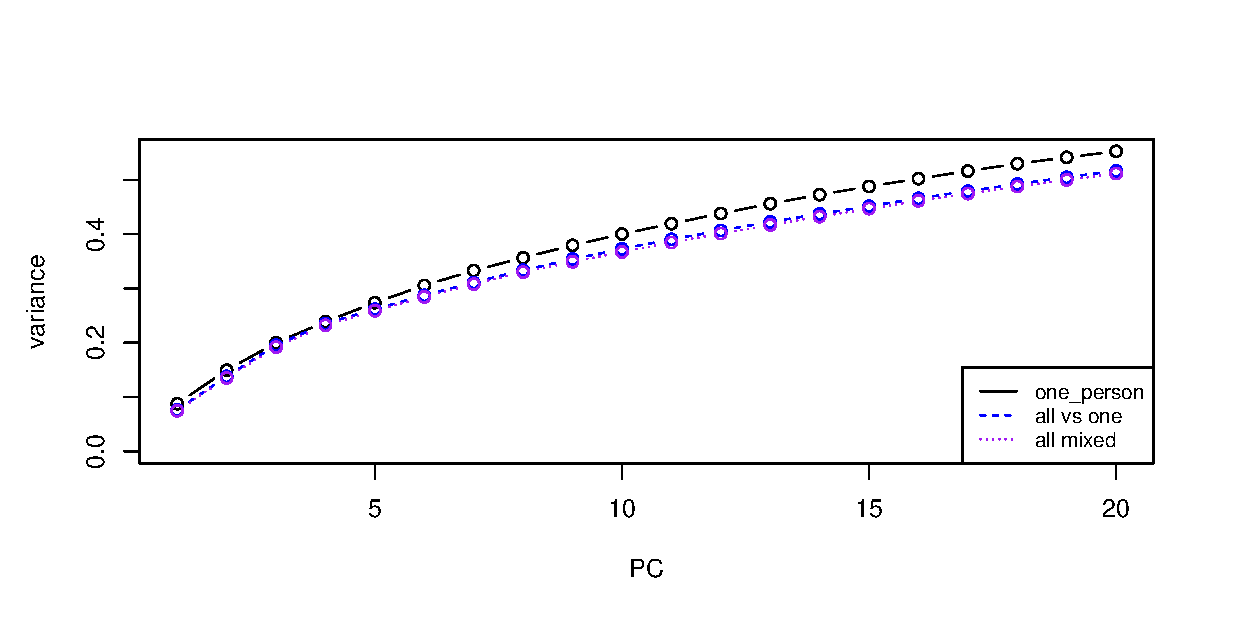
\includegraphics[width=\textwidth]{graphics/pca_acc_variance}
\caption{Accumulated variance}
\label{fig:pca_accumulated_var}
\end{subfigure}\\[-1cm]
\begin{subfigure}{0.70\textwidth}
\centering
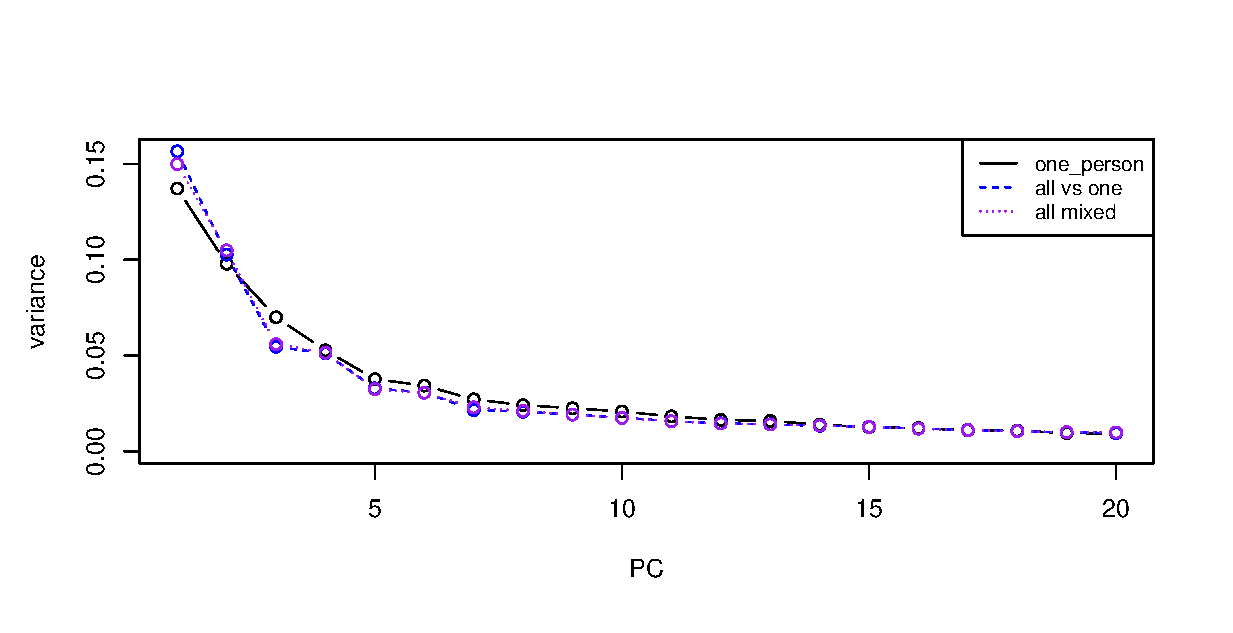
\includegraphics[width=\textwidth]{graphics/pca_variance}
\caption{Variance}
\label{fig:pca_accumulated_var}
\end{subfigure}
\caption[PCA variance]{Variance over the first 20 principle components.
The data was run on Group 3 member 2's data on 100 DPI. }
\label{fig:variance}
\end{figure}
% Figure \ref{fig:contour_KvsPCA_G3M2vsRest} shows a contour plot of how well Group 3 Member 2's  handwriting was predicted successfully for $K$ and the total variance represented of the PC's varying between one and 20 and 0.5 and 1 respectively.


Calculating with less data will result in a faster computation time.
Choosing too few PC means there is no features left to compare.
To see how the performance and the timing scales both are shown in figure \ref{fig:pca_timing}. K was chosen to be 10.
The success rate has a peak with a low set of attributes so there must be some confusion that gets sorted out. 

\begin{figure}[H]
\centering
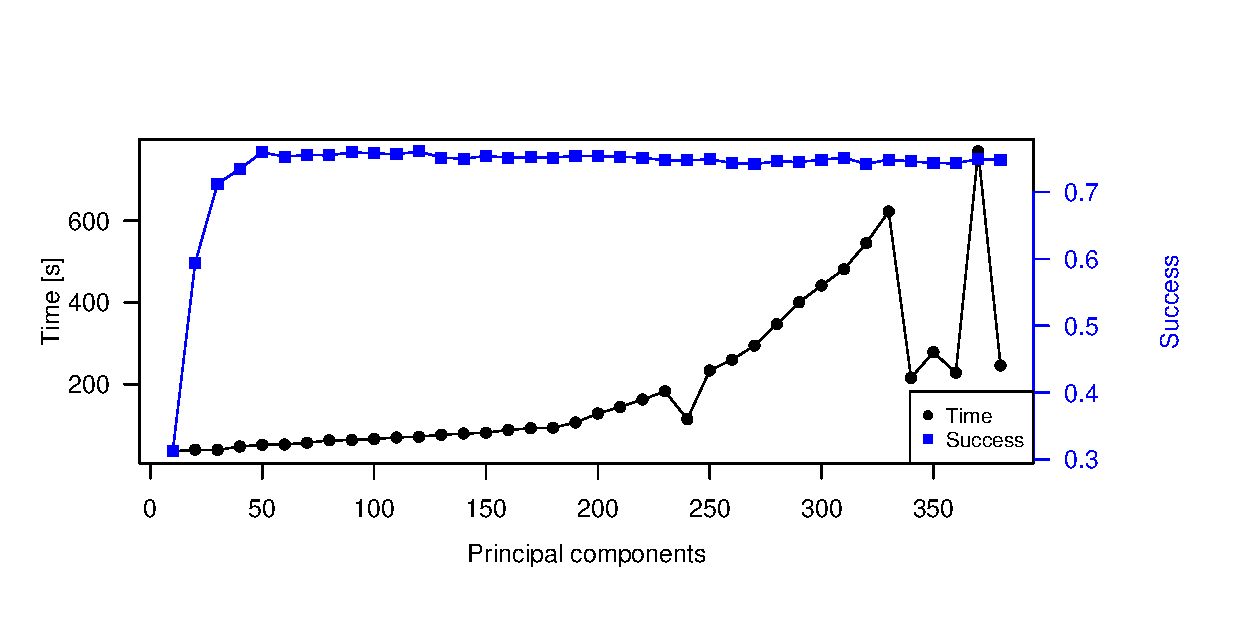
\includegraphics[width =0.8 \textwidth]{graphics/pca_timing}
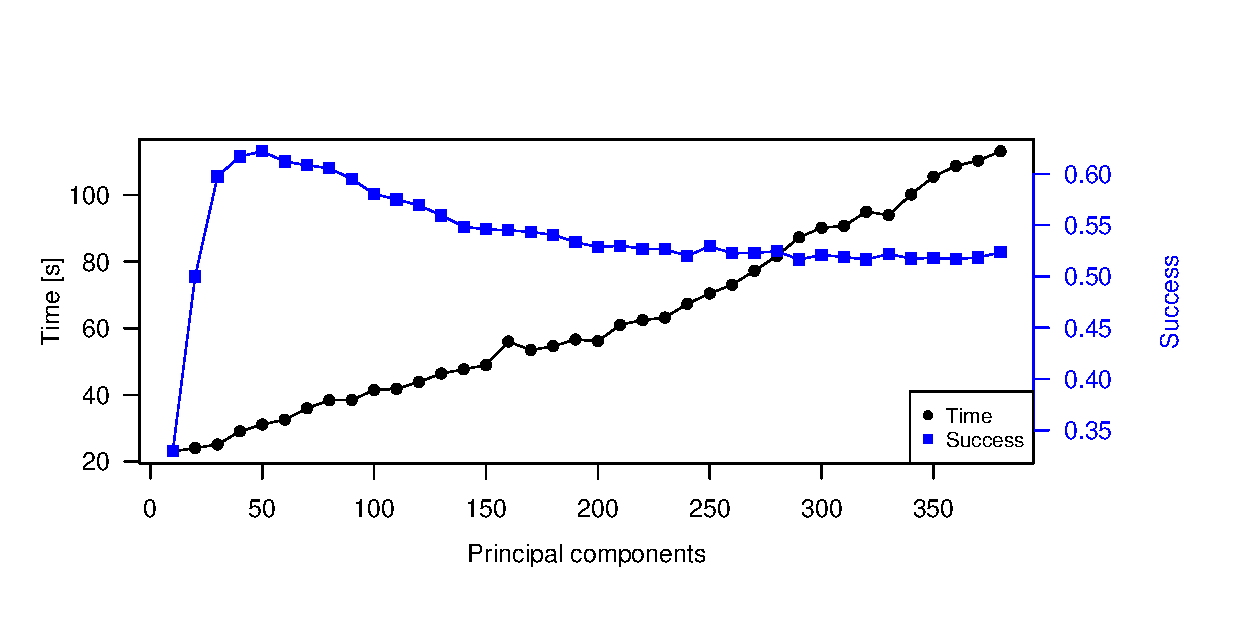
\includegraphics[width =0.8 \textwidth]{graphics/pca_timing_nikolaj}
\caption[Timing of PCA]{Timing of running the PCA with different principle components. 
The data was run on Group 3 member 2's data on 100 DPI. 
The percentage of successful predictions is also measured with the same data.}
\label{fig:pca_timing}
\end{figure}

To get a closer look at how the PCA performs the data from G3M2 was tested against the rest of the class. 
The K was chosen to be 10. 
The data is shown in figure \ref{fig:pca_success}.
The performance is getting worse as more features are considered.

\begin{figure}[H]
\centering
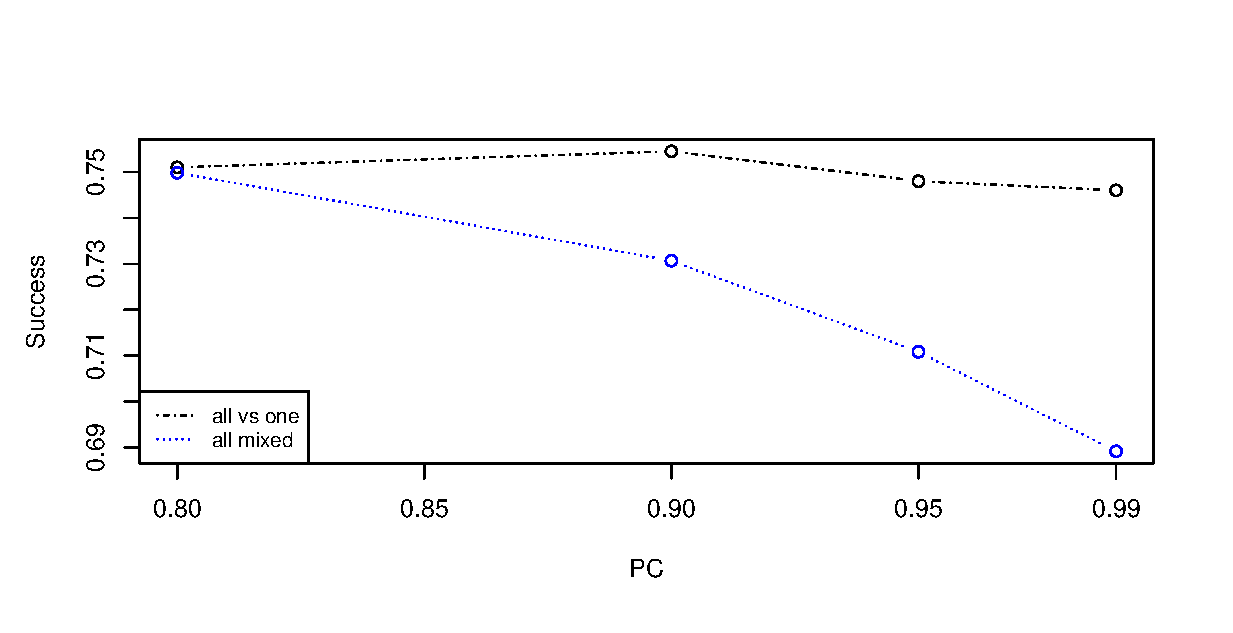
\includegraphics[width =0.95 \textwidth]{graphics/pca_success}
\caption[PCA performance]{Percentage of successful predictions with an increasing accumulated variance used.
The data was run on Group 3 member 2's vs data from 14 members on 100 DPI. Note that the axis are scaled.}
\label{fig:pca_success}
\end{figure}

To investigate the impact of K the test was redone so more K's were tested and that would lead to finding an optimum K for the large data set.
The data is shown in figure \ref{fig:k_v_PCA}. 
Where the optimum K was very small when testing a single person, a larger K is better suited for tests involving large data sets.
there still seems to be an optimum data size where the full data set performs worse than a smaller data set. 

\begin{figure}[H]
\centering
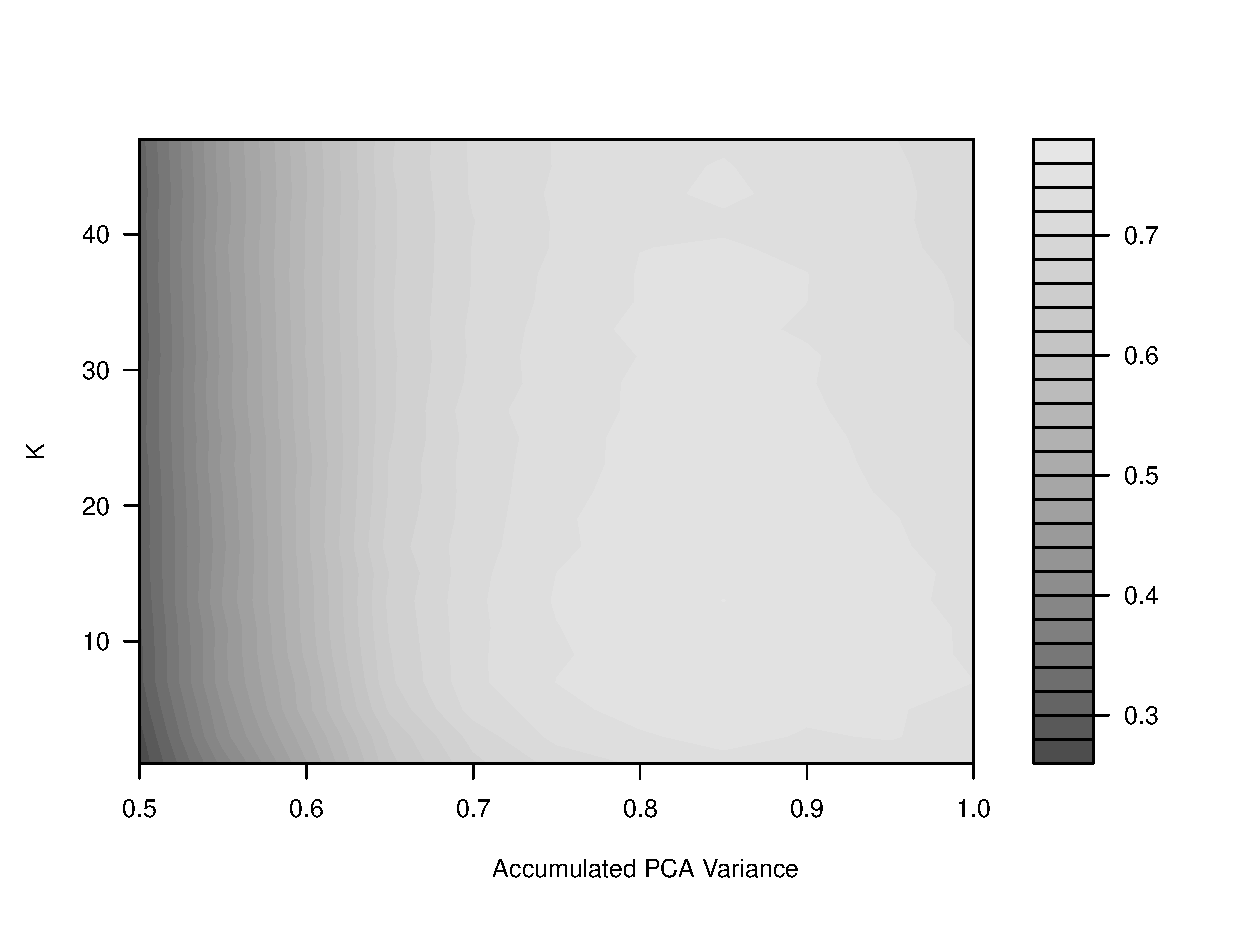
\includegraphics[width = \textwidth]{graphics/contour_k_PCA_oneVsRest}
\caption[Detailed PCA performance]{Success rate for detection of characters of Group 3 Member 2's data when he himself is not represented in the training set. 
The test was done with 16 people.}
\label{fig:k_v_PCA}
\end{figure}

As seen on figure \ref{fig:k_v_PCA}, then the optimum K and represented PCA variance is at $K = 10$ and $PCA = 0.8$. 
This is because an as high successful prediction rate is wanted, but also an as small dataset as possible. 
This point will further be used in section \ref{sec:DataNormalization}.

